\documentclass{beamer}

% \usepackage[utf8]{inputenc}
% \usepackage[T1]{fontenc}
\usepackage{lmodern}   % modern Latin Modern fonts
\usepackage{textcomp}  % provides \textquoteright
\usepackage{lmodern} % Latin Modern fonts with T1 shapes


\usepackage{graphicx}
\usepackage{ragged2e} % for generating dummy text
\usepackage[backend=biber,style=authoryear]{biblatex}
% \addbibresource{references.bib}

\usetheme{Madrid}
\usecolortheme{default}
\usefonttheme{professionalfonts} % keeps proper math fonts

\usepackage{amsmath,amssymb,amsfonts} % math symbols (\mathcal, \mathbb, etc.)
\usepackage{mathrsfs}                 % optional: \mathscr for fancy script

% \setbeamercovered{invisible} 
\setbeamercovered{transparent}



% \title{MF921 Topics in Dynamic Asset Pricing}
% \author{Stochastic Analysis \& Stochastic Calculus in Quantitative Finance}
% %\institute{Boston University}
% \date{Yuanhui Zhao\\Week 2\\Boston University}
\title{MF921 Topics in Dynamic Asset Pricing}
\subtitle{Stochastic Analysis \& Stochastic Calculus in Quantitative Finance}
\author{Yuanhui Zhao}
\date{Boston University \\ \;\;Week 2}

\begin{document}
\frame{\titlepage}
% \begin{frame}
% \frametitle{Outline}
% \tableofcontents
% \end{frame}
\section{Part I}
\begin{frame}{Part I, Chapter 15}
    \begin{center}
    Option
    Pricing via the Change of
    Numeraire Argument
    \end{center}
\end{frame}
\section{Change of Numeraire}
\begin{frame}{Change of Numeraire: Motivation and Key Idea}
    \par In option pricing, we usually price under the risk-neutral measure using 
    the money market account $B(t) = e^{rt}$ as the numeraire. 
    But sometimes payoffs become simpler if we change the unit of measurement (the numeraire).
    Instead of measuring in “dollars,” measure in “shares of stock”.
    \vspace{1em}
    \par The key idea is :
    \begin{itemize}
        \item Pick any strictly positive traded asset $N(t)$ as the numeraire.
        \item Then define a new probability measure $\tilde{\mathbb{P}}$ such that 
        $\frac{S(t)}{N(t)} \quad \text{is a martingale under } \tilde{\mathbb{P}}.$ No-arbitrage is preserved.
    \end{itemize}
    \vspace{1em}
    \par We first look at the details how this work (Radon Nikodym derivative \& Girsanov Theorem) and 
    then apply the scheme to price different type of options. 
\end{frame}
\begin{frame}{Change of Numeraire}
    \par Given $(\Omega, \mathcal{F}, (\mathcal{F}_t)_{t \geq 0}, \mathbb{P}^*)$ with $d$-dim Brownian $W$:
    \vspace{1em}
    \begin{itemize}
        \item Money market account (baseline numeraire): $ dB_t =  B_t r_t dt$
        \item Traded asset $S(t)$: $dS_t = S_t(r_t dt + \sigma_t\, dW_t),
    \quad \tfrac{S_t}{B_t} \text{ is a martingale.}$
        \item Derivative pricing rule: for payoff $X_T$ at maturity $T$, $V_0 = \mathbb{E}^{\mathbb{P}^*}\left[\frac{X_T}{B_T}\right]$
    \end{itemize}
    \vspace{1em}
    \par Our goal is to pick another strictly positive traded asset $N(t)$ and
  define a new measure $\tilde{\mathbb{P}}$ such that $\frac{S(t)}{N(t)}$ is a martingale for every traded asset $S(t)$.
\end{frame}
\begin{frame}{Change of Numeraire Con.}

    {\footnotesize \footnotesize
    \par Oberve $\displaystyle \frac{S(t)}{B(t)}$ is a martingale under $\mathbb{P}^*$. 
    We want $\displaystyle \frac{S(t)}{N(t)}$ to be a martingale under $\tilde{\mathbb{P}}$.
    \par Define $\tilde{\mathbb{P}}$ via the Radon$-$Nikodym derivative with respect to $\mathbb{P}^*$:
    \begin{align*}
        \left.\frac{d\tilde{\mathbb{P}}}{d\mathbb{P}^*}\right|_{\mathcal{F}_T} = Z_T : = \;\;\frac{N(T)/B(T)}{N(0)/B(0)}
    \end{align*}
    \par By construction, $\frac{N(T)}{B(T)}$ is a martingale under $\mathbb{P}^*$, $Z_T >0$ and $\mathbb{E}^{\mathbb{P}^*}[Z_T]=1$ and take any payoff $X_T$:
    \begin{align*}
         V(0) \;=\; N(0)\,\mathbb{E}^{\tilde{\mathbb{P}}}\!\left[\frac{X_T}{N(T)}\right] 
         =N(0) \mathbb{E}^{\mathbb{P}^*}\!\left[\frac{X_T}{N(T)}\,Z_T\right] = \mathbb{E}^{\mathbb{P}^*}\!\left[\frac{X_T}{B(T)}\right]
    \end{align*}
    \vspace{0.5em}
    \par So the choice of Radon$-$Nikodym derivative guarantees the prices are consistent under both measures and no arbitrage is preserved.
    }
    
\end{frame}
\begin{frame}{Change of Numeraire Con.}

    {\footnotesize \footnotesize
    \par What is the $dS(t)$ looks like under meausre $\tilde{\mathbb{P}}?$
    \par Note: Under $Q$, we have $\begin{cases}
        dS(t) = r(t) S(t) \,dt + \sigma(t) S(t) \,dW(t)\\dN(t) = r(t) N(t) \,dt + \gamma(t) N(t) \,dW(t)
    \end{cases}$
    \par Denote $\widehat N_t = \frac{N_t}{B_t}$, apply Itô we get
     $\frac{d\widehat N_t}{\widehat N_t}=\gamma_t\,dW_t$, $\widehat N_t
    = \widehat N_0 e^{\left(
      \int_0^t \gamma_s \cdot dW_s
      - \frac{1}{2} \int_0^t \|\gamma_s\|^2 \, ds
    \right)}.$
    \par Oberve that $Z_t  = \frac{\widehat N_t}{\widehat N_0} = e^{\left(
      \int_0^t \gamma_s \cdot dW_s
      - \frac{1}{2} \int_0^t \|\gamma_s\|^2 \, ds
    \right)}$
    \par Girsanov's theorem says: if we define a new measure $\tilde{\mathbb{P}}$ via this $Z_t$, then the process
            \[
        \tilde{W}(t) \;=\; W(t) - \int_{0}^{t}\gamma_sdt
            \]
        is a Brownian motion under $\tilde{\mathbb{P}}$. Substitute into $dS(t)$ to get the $\tilde{\mathbb{P}}$ dynamics:
        \begin{align*}
            dS(t) = S(t)\Big[ (r(t) + \sigma(t) \cdot \gamma(t))\,dt + \sigma(t)  \cdot d\tilde{W}(t) \Big]
        \end{align*}
        \begin{align*}
            S(t)
           = S_0 \exp\!\left(
            \int_0^t \!\Big(r(s) + \sigma(s) \!\cdot\!\gamma(s) - \tfrac12 \|\sigma(s)\|^2\Big) ds
            + \int_0^t \!\sigma(s) \!\cdot\! d\tilde{W}(s)\right)
        \end{align*}
    }
    
\end{frame}
\section{Black-Scholes Formula}
\begin{frame}{Black-Scholes Formula}


    {\footnotesize \footnotesize
    \par Given $r, \sigma$ are constant, we have $S(T) = S(0) \exp\left\{(r - \tfrac{1}{2} \sigma^2) T + \sigma W(T)\right\}$.
    \vspace{1em}
    \par The no-arbitrage price for the call option:
    \begin{align*}
        \psi_c(0)& = \mathbb{E}^{\mathbb{P}^*}(e^{-rT}(S(T) - K)^+)\\&= \mathbb{E}^{\mathbb{P}^*}(e^{-rT}(S(T) - K)I(S(T) \geq K)) \\
        &= \mathbb{E}^{\mathbb{P}^*}(e^{-rT}S(T)I(S(T) \geq K)) - Ke^{-rT}\mathbb{P}^*(S(T) \geq K)\\& = I - Ke^{-rT} \cdot II \
    \end{align*}
    \par For $II$:
    \begin{align*}
        II = \mathbb{P}^*(S(T) \geq K) &= 1 - \Phi \left( \frac{\log(K/S(0)) - (r - \frac{1}{2}\sigma^2)T}{\sigma\sqrt{T}} \right) \\
        &= \Phi \left( \frac{\log(S(0)/K) + (r - \frac{1}{2}\sigma^2)T}{\sigma\sqrt{T}} \right)
    \end{align*}
    \par Note: $\Phi$ is the CDF of the standard normal distribution.
    }
\end{frame}
\begin{frame}{Black-Scholes Formula Con.}

    {\footnotesize \footnotesize
    \par For $I$, we apply the change of numeraire and use stock itself as numeraire. Then based on the eraly definition
    we have $\left.\frac{d\tilde{\mathbb{P}}}{d\mathbb{P}^*}\right|_{\mathcal{F}_T} = Z_T :=  e^{-rT}\frac{S(T)}{S(0)}$
    and $\gamma_t = \sigma$. Therefore, under \(\tilde{\mathbb{P}}\) we have the following dynamics of \(S(t)\):
    \[
    \frac{dS_t}{S_t} = rdt + \sigma^2 dt + \sigma \tilde{dW_t},\;
    S(t) = S(0) \exp \left\{ (r + \sigma^2/2) t + \sigma \tilde{W_t} \right\}
    \]
    \par Then we can rewrite $I$:
    \begin{align*}
        I = S(0)\mathbb{E}^{\mathbb{P}^*} \left( e^{-rT} \frac{S(T)}{S(0)} I(S(T) \geq K) \right) &= S(0) \mathbb{E}^{\tilde{\mathbb{P}}} (I(S(T) \geq K)) \\
        &= S(0) \tilde{\mathbb{P}}(S(T) \geq K)\\
       & = S(0) \Phi \left( \frac{\log(S(0)/K) + (r + \frac{1}{2} \sigma^2) T}{\sigma \sqrt{T}} \right).
    \end{align*}
   \par Putting together, we have the price of the call option is given by:
    \[
    I - Ke^{-rT} \cdot II = S(0) \Phi(d_+) - Ke^{-rT} \Phi(d_-)
    \]
where $d_{\pm} = \frac{\log(S(0)/K) + (r \pm \frac{1}{2} \sigma^2) T}{\sigma \sqrt{T}}.$

    }
\end{frame}

\section{One Dimensional Barrier Options}
\begin{frame}{One Dimensional Barrier Options}

    {\footnotesize \footnotesize
    \par Barrier options are path-dependent derivatives whose payoff is activated (knock-in) or extinguished (knock-out) 
    if the underlying asset crosses a pre-specified barrier. They extend vanilla 
    calls/puts by adding a barrier condition.
    \par We first study continuously monitored barriers and derive 
    Merton's closed-form pricing formulas (1973) for single-barrier options.
    \par Given $(\Omega, \mathcal{F}, (\mathcal{F}_t)_{t \geq 0}, \mathbb{P}^*)$ with 1-dim Brownian $W$. 
    The Market setting following:
    \begin{align*}
        dB(t) =  B(t) r dt\;,\;dS(t) = r S(t)  dt + \sigma S(t)  dW(t)
    \end{align*}
    % \begin{center}
    %     $\begin{cases}
    %     dB_t =  B_t r dt\\ 
    % \end{cases}$
    % \end{center}
    \par A continuously monitored barrier option has 
    payoff = vanilla option payoff \(\times\) indicator of the barrier condition. For example: 
    \begin{itemize}
        \item Up-and-out call: $V_0 = \mathbb{E}^{\mathbb{P}^*} \left[ e^{-rT} (S(T) - K)^+ I{\left\{ \max\limits_{0 \leq t \leq T} S(t) \leq H \right\}} \right], \quad H > S(0)$
        \item Down-and-in put: $ V_0 = \mathbb{E}^{\mathbb{P}^*} \left[ e^{-rT} (K - S(T))^+ I{\left\{ \min\limits_{0 \leq t \leq T} S(t) \leq H \right\}} \right], \quad H < S(0)$
    \end{itemize}
     \par Study the case of the down-and-in call option (DAIC) with strike \( K \), barrier \( H < S(0) \):
    \begin{align*}
        \text{DAIC} = e^{-rT}  \mathbb{E}^{\mathbb{P}^* }
        \left[ (S(T) - K)^+ I{\left\{\min\limits_{0 \leq t \leq T} S(t) \leq H \right\}} \right] 
    \end{align*}
    }
    
\end{frame}
\begin{frame}{One Dimensional Barrier Options Con.}
    
    {\footnotesize \footnotesize
    \par For notation simplicity, denote a drifted Brownian motion:
          \[
          W_{\mu,\sigma}(t) = \mu t + \sigma W(t), \quad M_t = \max_{0 \leq s \leq t} W_{\mu,\sigma}(s).
          \]
    \par Some useful results from the reflection principle for a Brownian motion with a  drift:
    \par (i) When \( x \leq y \), $y > 0,  \sigma > 0$ :
    \begin{itemize}
         {\footnotesize \scriptsize
        \item $P(W_{\mu, \sigma}(t) \leq x,  M_t \geq y) = e^{2\mu y / \sigma^2} 
        \Phi \left( \frac{x - 2y - \mu t}{\sigma \sqrt{t}} \right)$
        \item $P(W_{\mu, \sigma}(t) \leq x,  M_t \leq y) = \Phi \left( \frac{x - \mu t}{\sigma \sqrt{t}} \right) - e^{2\mu y / \sigma^2} 
         \Phi \left( \frac{x - 2y - \mu t}{\sigma \sqrt{t}} \right)$
         }
    \end{itemize}
    \par (ii) When \( x \geq y>0 \), $\sigma > 0$:
    \begin{itemize}
         {\footnotesize \scriptsize
        \item $P(W_{\mu, \sigma}(t) \leq x,  M_t \leq y) = P(M_t \leq y) \nonumber =
            \Phi \left( \frac{y - \mu t}{\sigma \sqrt{t}} \right) - e^{2\mu y / \sigma^2} \Phi 
            \left( \frac{-y - \mu t}{\sigma \sqrt{t}} \right)$
        \item $P(W_{\mu, \sigma}(t) \leq x,  M_t \geq y) = P(W_{\mu, \sigma}(t) \leq x) - P(W_{\mu, \sigma}(t) \leq x,  M_t \leq y) \nonumber 
            = \Phi \left( \frac{x - \mu t}{\sigma \sqrt{t}} \right) - 
            \Phi \left( \frac{y - \mu t}{\sigma \sqrt{t}} \right) + e^{2\mu y / \sigma^2} \Phi \left( \frac{-y - \mu t}{\sigma \sqrt{t}} \right)$
         }
    \end{itemize}
    \par (iii) When \( x \geq y \), $y < 0$, $\sigma > 0$:
    \begin{itemize}{\footnotesize \scriptsize
        \item $P\left( W_{\mu, \sigma}(t) \geq x, \min\limits_{0 \leq s \leq t} W_{\mu, \sigma}(s) \leq y \right) 
        = e^{2\mu y / \sigma^2} \Phi \left( \frac{-x + 2y + \mu t}{\sigma \sqrt{t}} \right)$
        }
    \end{itemize}
    }
\end{frame}
\begin{frame}{One Dimensional Barrier Options Con.}

    {\footnotesize \scriptsize
    \par Back to the valuation of DAIC:
    {\footnotesize \scriptsize
    \begin{align*}
    &\mathbb{E}^{\mathbb{P}^*}\left[e^{-rT}(S(T) - K)^+ I\left(\min_{0 \leq t \leq T} S(t) \leq H\right)\right]\\
    &= \mathbb{E}^{\mathbb{P}^*}\left[e^{-rT}(S(T) - K)I\left(S(T) \geq K, \min_{0 \leq t \leq T} S(t) \leq H\right)\right] \\
    &= \mathbb{E}^{\mathbb{P}^*}\left[e^{-rT}S(T)I\left(S(T) \geq K, \min_{0 \leq t \leq T} S(t) \leq H\right)\right] \\
    &\quad - Ke^{-rT}P^*\left(S(T) \geq K, \min_{0 \leq t \leq T} S(t) \leq H\right) \\
    &= I - Ke^{-rT} \cdot II 
    \vspace{-0.5em}
    \end{align*}
    \par For II:
    \vspace{-0.5em}
    \begin{align*}
    II &= P^*\left(S(T) \geq K, \min_{0 \leq t \leq T} S(t) \leq H\right) \\
    &= P\left\{W_{r-\frac{\sigma^2}{2},\sigma}(T) \geq \log(K/S(0)), \min_{0 \leq t \leq T} W_{r-\frac{\sigma^2}{2},\sigma}(t) \leq \log(H/S(0))\right\} \\
    &= \exp\left\{\frac{2(r - \sigma^2/2)}{\sigma^2} \log(H/S(0))\right\} 
     \cdot \Phi \left(\frac{2 \log(H/S(0)) - \log(K/S(0)) + (r - \sigma^2/2)T}{\sigma \sqrt{T}}\right)\\
     &=(H/S(0))^{\frac{2r}{\sigma^2}-1} \Phi \left(\frac{\log(\{H^2/S(0)\}/K) 
     + (r - \sigma^2/2)T}{\sigma \sqrt{T}}\right)\\
    \end{align*}

    }
    }
\end{frame}
\begin{frame}{One Dimensional Barrier Options Con.}
    
    {\footnotesize \footnotesize
    \par For I, by changing of numeraire we can get:
    \vspace{-0.5em}
    {\footnotesize \scriptsize
    \begin{align*}
    I &= S(0) \mathbb{E}^{\mathbb{P}^*} \left( e^{-rT} \frac{S(T)}{S(0)} \cdot I\left\{S(T) \geq K, \min_{0 \leq t \leq T} S(t) \leq H\right\} \right) \\
    &= S(0) \tilde{P}\left(S(T) \geq K, \min_{0 \leq t \leq T} S(t) \leq H\right) \\
    &= S(0) P\left\{W_{r+\frac{\sigma^2}{2}, \sigma}(T) \geq \log(K/S(0)), \min_{0 \leq t \leq T} W_{r+\frac{\sigma^2}{2}, \sigma}(t) \leq \log(H/S(0))\right\} \\
    &= S(0) \cdot (H/S(0))^{\frac{2r}{\sigma^2}+1} \Phi \left( \frac{\log(\{H^2/S(0)\}/K)+(r+\sigma^2/2)T}{\sigma\sqrt{T}} \right) \\
    &= (H/S(0))^{\frac{2r}{\sigma^2}-1}(H^2/S(0)) \Phi \left( \frac{\log(\{H^2/S(0)\}/K)+(r+\sigma^2/2)T}{\sigma\sqrt{T}} \right)
    \end{align*}
    \par Putting the two terms together, we get $I - Ke^{-rT} \cdot II = (H/S(0))^{\frac{2r}{\sigma^2}-1} \text{BSC}(H^2/S(0))$. 
    Where \(\text{BSC}(x)\) is the Black-Scholes formula for a call option with the initial stock price being \(x\):
    \begin{align*}
        \text{BSC}(x) = x\Phi(d_+) - Ke^{-rT}\Phi(d_-) \text{ with } d_{\pm} = \frac{\log(x/K)+(r\pm\sigma^2/2)T}{\sigma\sqrt{T}}
    \end{align*}
    \vspace{-1em}
    }
    }
\end{frame}
\section{Exchange Options}
\begin{frame}{Exchange Options}

    {\footnotesize \footnotesize
    \par Given $(\Omega, \mathcal{F}, (\mathcal{F}_t)_{t \geq 0}, \mathbb{P}^*)$ 
    with 2-dim independent Brownian, \( W_1(t) \) and \( W_2(t) \). 
    We have two traded assets \( S_1(t) \) and \( S_2(t) \) with the following dynamics:
    \begin{align*}
    \frac{dS_1(t)}{S_1(t)} &= rdt + \sigma_1 dW_1(t) \\
    \frac{dS_2(t)}{S_2(t)} &= rdt + \sigma_2 \left\{ \rho dW_1(t) + \sqrt{1 - \rho^2} dW_2(t) \right\}
    \end{align*}
    \par The exchange option gives the holder the right, but not the obligation, 
    to exchange asset \(S_2\) for asset \(S_1\) at maturity \(T\). The price of this option as following:
    \begin{align*}
        u(0) &= \mathbb{E}^{\mathbb{P}^*}\left[e^{-rT}(S_1(T) - S_2(T))^+\right]\\
        &=S_2(0) \mathbb{E}^{\mathbb{P}^*}\left[ \frac{e^{-rT} S_2(T)}{S_2(0)} \left( \frac{S_1(T)}{S_2(T)} - 1 \right)^+ \right] \\
        &= S_2(0) \mathbb{E}^{\tilde{\mathbb{P}}} \left[ \left( \frac{S_1(T)}{S_2(T)} - 1 \right)^+ \right] \\
        &= S_2(0) \mathbb{E}^{\tilde{\mathbb{P}}} \left[ (F(T) - 1)^+ \right]
    \end{align*}

    }
\end{frame}
\begin{frame}{Exchange Options Con.}

    {\footnotesize \footnotesize
    \par Apply Itô, we have the Radon$-$Nikodym derivative for numeraire:
    \begin{align*}
        \left.\frac{d\tilde{\mathbb{P}}}{d\mathbb{P}^*}\right|_{\mathcal{F}_T}& = Z_T^2 := \frac{e^{-rT} S_2(T)}{S_2(0)} = \exp \left[ \sigma_2 
        \left\{ \rho W_1(T) + \sqrt{1 - \rho^2} W_2(T) \right\} - \frac{T}{2} \sigma_2^2 \right]\\
        \left.\frac{d\hat{\mathbb{P}}}{d\mathbb{P}^*}\right|_{\mathcal{F}_T}& = Z_T^1 := \frac{e^{-rT} S_1(T)}{S_1(0)} 
        =\frac{e^{-rT}S_1(T)}{S_1(0)} = \exp\left(\sigma_1 W_1(T) - \frac{1}{2}\sigma_1^2 T\right)\\
    \end{align*}

    \vspace{-2em}
    \par By Girsanov theorem, under new measure $\tilde{\mathbb{P}}$:
    \begin{align*}
        \tilde{W}_1(t) &= W_1(t) - \rho\sigma_2 t, \;\; \tilde{W}_2(t) = W_2(t) - \sigma_2\sqrt{1-\rho^2} t
    \end{align*}
    \par Apply Itô, we can get $d\ln S_1$, $d\ln S_2$:
    \begin{align*}
        d \ln F(t) &= d \ln S_1(t) - d \ln S_2(t) \\
        &= \left[  - \tfrac{1}{2}\sigma_1^2  - \tfrac{1}{2}\sigma_2^2 + \rho \sigma_1 \sigma_2 \right] dt 
        + (\sigma_1 - \rho \sigma_2) d\tilde{W}_1 - \sigma_2 \sqrt{1-\rho^2} d\tilde{W}ߢ_2.
    \end{align*}
    \par Apply Itô to $g(x) = e^x$ with $x = \ln F(t)$:
    \begin{align*}
        \frac{dF_t}{F_t} = d(\ln F_t) + \frac{1}{2} d<\ln F>_t 
        = (\sigma_1 - \rho\sigma_2) d\tilde{W}_{1t} - \sigma_2 \sqrt{1 - \rho^2} d\tilde{W}_{2t}
    \end{align*}
    }
\end{frame}
\begin{frame}{Exchange Options Con.}
    
    {\footnotesize \footnotesize
    \par Denote $\sigma  = \sqrt{\sigma_1^2 - 2\rho\sigma_1\sigma_2 + \sigma_2^2}$, $\tilde{W}(t) := \frac{1}{\sigma} \left\{ (\sigma_1 - \rho\sigma_2)\tilde{W}_1(t) - \sigma_2\sqrt{1 - \rho^2}\tilde{W}_2(t) \right\}$
    Observe that $\tilde{W}$ is a standard Brownian motion under $\tilde{\mathbb{P}}$. 
    We have $\frac{dF(t)}{F(t)} = \sigma d\tilde{W}(t)$, observe that $F_T = F_0 \exp \left( - \frac{1}{2} \sigma^2 T 
    + \sigma \sqrt{T} Z \right),  Z \sim N(0, 1)$ under $\tilde{\mathbb{P}}$. Similarly, we have 
    $F_T = F_0 \exp \left(  \frac{1}{2} \sigma^2 T 
    + \sigma \sqrt{T} Z \right),  Z \sim N(0, 1)$ under $\hat{\mathbb{P}}$.
    \vspace{1em}
    % and \(\ln F_T \sim N(\ln F_0 - \frac{1}{2} \sigma^2 T, \sigma^2 T)\).
     \par Then we can rewrite $u(0)$:
     
     \begin{align*}
        u(0) &= S_2(0) \mathbb{E}^{\tilde{\mathbb{P}}} \left[ (F(T) - 1)^+ \right]\\
        &= S_2(0) \mathbb{E}^{\tilde{\mathbb{P}}} \left[ (F(T) - 1)I(F(T)>1) \right]\\
        &=S_2(0) \left[ \mathbb{E}^{\tilde{\mathbb{P}}}[F_T I{\{F_T > 1\}}] 
        - \tilde{\mathbb{P}}(F_T > 1)\right] \\
        &=S_2(0) \left[ \mathbb{E}^{\mathbb{P}^*}[\frac{e^{-rT} S_2(T)}{S_2(0)} \frac{S_1(T)}{S_2(T)} I{\{F_T > 1\}}] 
        - \tilde{\mathbb{P}}(F_T > 1)\right] \\
        &=S_2(0) \left[ \frac{1}{S_2(0)}\mathbb{E}^{\mathbb{P}^*}[\frac{e^{-rT} S_1(T)}{S_1(0)} S_1(0) I{\{F_T > 1\}}] 
        - \tilde{\mathbb{P}}(F_T > 1)\right] \\
     \end{align*}
    
    }

\end{frame}
\begin{frame}{Exchange Options Con.}
    
    {\footnotesize \footnotesize   
    \begin{align*}
        = &  S_2(0) \left[ \frac{S_1(0)}{S_2(0)}\mathbb{E}^{\hat{\mathbb{P}}}[ I{\{F_T > 1\}}] 
        - \tilde{\mathbb{P}}(F_T > 1)\right] \\
        = & S_1(0)\hat{\mathbb{P}}[ I{\{F_T > 1\}}] 
        - S_2(0)\tilde{\mathbb{P}}(F_T > 1) \\
        = & S_1(0) \Phi (d_+) - S_2(0) \Phi (d_-) \\
    \end{align*}
    \par Where:
    \begin{align*}
        d_\pm = \frac{\log(F(0)) \pm \frac{1}{2} \sigma^2 T}{\sigma \sqrt{T}} 
        = \frac{\log(S_1(0)/S_2(0)) \pm \frac{1}{2} \sigma^2 T}{\sigma \sqrt{T}}.
    \end{align*}
    \begin{itemize}
        \item (i) If the second asset is cash, or \( S_2(t) = Ke^{-r(T-t)} \), 
        then the formula degenerates to the Black-Scholes formula.
        \item (ii) The hedging strategy is given by long \( \Phi(d_+) \) 
        shares of the first asset and short \( \Phi(d_-) \) shares of the second asset.
    \end{itemize}
    }
    
\end{frame}
\section{Two-Dimensional Barrier Options}
\begin{frame}{Two-Dimensional Barrier Options}
    
    {\footnotesize \footnotesize
    \par Suppose we have two Wiener processes, \( X(t) \) and \( Y(t) \), governed by the following dynamics
    \begin{align*}
    dX(t) &= \mu_1 dt + \sigma_1 dW_1(t), \quad X(0) = 0, \quad \sigma_1 > 0, \\
    dY(t) &= \mu_2 dt + \sigma_2 \left\{ \rho dW_1(t) + \sqrt{1 - \rho^2} dW_2(t) \right\}, \quad Y(0) = 0, \quad \sigma_2 > 0,
    \end{align*}
    \par where the \( W_1 \) and \( W_2 \) are two independent standard Brownian motions.
    \par For \( b > 0 \), consider the first passage time of the process \( Y(t) \):
    \[
    \tau_b^Y = \inf\{t \geq 0: Y(t) = b > 0\}.
    \]
    \par We shall prove that the joint distribution between \( X(T) \) and the first passage time of \( Y(t) \) is given by:
    \vspace{-1em}
    \begin{align*}
    &P(X(T) < a, \tau_b^Y > T) = P\left(X(T) < a, \max_{0 \leq t \leq T} Y(t) < b\right) \\
    = \Phi_2 & \left( \frac{a - \mu_1 T}{\sigma_1 \sqrt{T}}, \frac{b - \mu_2 T}{\sigma_2 \sqrt{T}} ; \rho \right) - 
    e^{2 \mu_2 b / \sigma_2^2} \Phi_2 \left( \frac{a - \mu_1 T - 2 \rho b \sigma_1 / \sigma_2}{\sigma_1 \sqrt{T}}, \frac{-b - \mu_2 T}{\sigma_2 \sqrt{T}} ; \rho \right)
    \end{align*}
    where $b > 0$ and \( \Phi_2(x, y; \rho) \) denotes the bivariate normal distribution given by
    \[
    \Phi_2(x, y; \rho) = P(Z_1 \leq x, Z_2 \leq y),
    \]
    with \( Z_1 \) and \( Z_2 \) being two standard normal random variables with correlation \( \rho \).
    \vspace{1em}

    }

\end{frame}

\begin{frame}{Two-Dimensional Barrier Options Con.}
    
    {\footnotesize \footnotesize
    \par Remark:
    \begin{itemize}
        \item Above equation holds for both \( a \geq b \) and \( a \leq b \), as long as \( b > 0 \).
        That's more general than the 1D reflection principle formulas which needed to be split into 
        separate cases depending on $a \leq b$ or $a \geq b$. 
        \item when \( \rho = 1 \), \( \mu_1 = \mu_2 = \mu \), \( \sigma_1 = \sigma_2 = \sigma \), 
        the two dimensional case reduces to the one-dimensional case, as it becomes:
        {\footnotesize \scriptsize
        \begin{align*}
        &P\left(X(T) < a, \max_{0 \leq t \leq T} X(t) < b\right) \\
        &= \Phi_2 \left( \frac{a - \mu T}{\sigma \sqrt{T}}, \frac{b - \mu T}{\sigma \sqrt{T}}; 1 \right) - e^{2\mu b / \sigma^2} \Phi_2 \left( \frac{a - \mu T - 2b}{\sigma \sqrt{T}}, \frac{-b - \mu T}{\sigma \sqrt{T}}; 1 \right) \\
        &= P \left\{ Z \leq \frac{a - \mu T}{\sigma \sqrt{T}}, Z \leq \frac{b - \mu T}{\sigma \sqrt{T}} \right\}
         - e^{2\mu b / \sigma^2} P \left\{ Z \leq \frac{a - \mu T - 2b}{\sigma \sqrt{T}}, Z \leq \frac{-b - \mu T}{\sigma \sqrt{T}} \right\}\\
        &=P \left\{ Z \leq \min\left\{\frac{a - \mu T}{\sigma \sqrt{T}}, \frac{b - \mu T}{\sigma \sqrt{T}}\right\} \right\}
         - e^{2\mu b / \sigma^2} P \left\{ Z \leq \min\left\{\frac{a - \mu T - 2b}{\sigma \sqrt{T}},\frac{-b - \mu T}{\sigma \sqrt{T}}\right\}  \right\}\\
        \end{align*}
        }
        \par Which incorporates two cases in one dimensional case.
    \end{itemize}
    }

\end{frame}

\begin{frame}{Two-Dimensional Barrier Options Con.}

    {\footnotesize \footnotesize
    Next we proof the formula of the joint distribution between \( X(T) \) 
    and the first passage time of \( Y(t) \):
    \par [Proof]
    \par Consider the case of $\sigma_1 = \sigma_2 = 1$. Define a new process $V(t)$ to decouple $X$ and $Y$:
    \begin{align*}
        V(t) := X(t) - \rho Y(t)
    \end{align*}
    \par First check independence between $V$ and $Y$:
    \begin{align*}
        dV(t)  dY(t)  & = (dX(t) - \rho  dY(t))  dY(t)\\
        &= \left( (1 - \rho^2) dW_1 - \rho \sqrt{1 - \rho^2}  
        dW_2 \right) \cdot \left( \rho dW_1 + \sqrt{1 - \rho^2}  dW_2 \right)\\
        &=(1 - \rho^2) \rho (dW_1)^2 - \rho (1 - \rho^2) (dW_2)^2\\
        &= (1 - \rho^2) \rho dt - (1 - \rho^2) \rho dt = 0
    \end{align*}
    \par  Since \( V(T) = X(T) - \rho Y(T) \), it is Gaussian. Its mean is:
    \begin{align*}
        \mathbb{E}[V(T)] = \mu_1 T - \rho \mu_2 T
    \end{align*}
    }
\end{frame}
\begin{frame}{Two-Dimensional Barrier Options Con.}

    {\footnotesize \footnotesize
    \par Its variance is:
    \begin{align*}
        \text{Var}(V(T)) 
        &= \text{Var}(X(T)) + \rho^2 \text{Var}(Y(T)) - 2\rho \text{Cov}(X(T), Y(T))\\
        &= T + \rho^2 T - 2\rho^2 T = (1 - \rho^2)T\\
    \end{align*}
    \par Thus:
        \[
        V(T) \sim N((\mu_1 - \rho \mu_2)T, (1 - \rho^2)T).
        \]
    \par Incidentally, the same logic applying to two standard normal random variables with correlation \(\rho\) also leads to a representation for the bivariate normal distribution:
    \[
    \Phi_2(\alpha, \beta; \rho) = \int_{z_2=-\infty}^{\beta} \int_{z_1=-\infty}^{\alpha} \frac{1}{\sqrt{1 - \rho^2}} \varphi\left( \frac{z_1 - \rho z_2}{\sqrt{1 - \rho^2}} \right) \varphi(z_2) \, dz_1 \, dz_2.
    \]
    \par Where $\varphi(\cdot)$ is the standard normal density function, $\varphi(z) = \frac{1}{\sqrt{2\pi}}\exp\left(-\frac{z^2}{2}\right).$

    }
    
\end{frame}
\begin{frame}{Two-Dimensional Barrier Options Con.}

    {\footnotesize \footnotesize
    \par Now, in terms of \(V(T)\), we can rewrite \(P(X(T) < a,  \tau_b^Y > T)\) as:
        \begin{align*}
        &P(X(T) < a,  \tau_b^Y > T) \\
        &= \int_{x=-\infty}^{a} \int_{y=-\infty}^{b} P(X(T) \in dx,  Y(T) \in dy,  \tau_b^Y > T) \\
        &\text{Note:the transformation is linear with determinant 1 and the independence of \(V\) and \(Y\)}\\
        &= \int_{x=-\infty}^{a} \int_{y=-\infty}^{b} P(V(T) \in dx - \rho dy) P(Y(T) \in dy,  \tau_b^Y > T)
        \end{align*}
    \par There are two terms inside the integrand. For the first term since \( V(T) \) has a normal distribution with mean \( \mu_1 T - \rho \mu_2 T \) 
    and variance \( (1 - \rho^2)T \), we have:
        \[
        P(V(T) \in dx - \rho dy) = \frac{1}{\sqrt{(1 - \rho^2)T}} \varphi \left( \frac{x - \rho y - \mu_1 T + \rho \mu_2 T}{\sqrt{(1 - \rho^2)T}} \right),
        \]
    }
\end{frame}
    
\begin{frame}{Two-Dimensional Barrier Options Con.}

    {\footnotesize \footnotesize
    \par For the second term, recall the eraly result in one-dim, When \( x \leq y \), $y > 0,  \sigma > 0$:
    \begin{align*}
        P(W_{\mu, \sigma}(t) \leq x,  M_t \leq y) = \Phi \left( \frac{x - \mu t}{\sigma \sqrt{t}} \right) - e^{2\mu y / \sigma^2} 
         \Phi \left( \frac{x - 2y - \mu t}{\sigma \sqrt{t}} \right)
    \end{align*}
    \par We have for all \( y < b,  b > 0 \):
            \[
        P(Y(T) \leq y,  \tau_b^Y > T) = \Phi \left( \frac{y - \mu_2 T}{\sqrt{T}} \right) - e^{2\mu_2 b} \Phi \left( \frac{y - 2b - \mu_2 T}{\sqrt{T}} \right).
        \]
    \par Differentiating the above equation yields:
        \[
        P(Y(T) \in dy,  \tau_b^Y > T) = \frac{1}{\sqrt{T}} \varphi \left( \frac{y - \mu_2 T}{\sqrt{T}} \right) - \frac{1}{\sqrt{T}} e^{2\mu_2 b} \varphi \left( \frac{y - 2b - \mu_2 T}{\sqrt{T}} \right).
        \]
    \par  Plugging the above two terms into:
    \begin{align*}
        \int_{x=-\infty}^{a} \int_{y=-\infty}^{b} P(V(T) \in dx - \rho dy) P(Y(T) \in dy,  \tau_b^Y > T)
    \end{align*}
    }

\end{frame}
\begin{frame}{Two-Dimensional Barrier Options Con.}

    {\footnotesize \footnotesize
    \begin{align*}
        P(X(T)<a, \tau_b^Y >T)=I - II
    \end{align*}
    \par where:
     {\footnotesize \tiny
    \begin{align*}
        I &= \int_{x=-\infty}^a \int_{y=-\infty}^b \frac{1}{\sqrt{(1-\rho^2)T}} \varphi \left( \frac{x-\rho y-\mu_1 T+\rho\mu_2 T}{\sqrt{(1-\rho^2)T}} \right) \frac{1}{\sqrt{T}} \varphi \left( \frac{y-\mu_2 T}{\sqrt{T}} \right) dy dx, \\
        II &= e^{2\mu_2 b} \int_{x=-\infty}^a \int_{y=-\infty}^b \frac{1}{\sqrt{(1-\rho^2)T}} \varphi \left( \frac{x-\rho y-\mu_1 T+\rho\mu_2 T}{\sqrt{(1-\rho^2)T}} \right) \frac{1}{\sqrt{T}} \varphi \left( \frac{y-2b-\mu_2 T}{\sqrt{T}} \right) dy dx,
        \end{align*}
    
     }
     \par and \(\varphi(x)=e^{-x^2/2}/\sqrt{2\pi}\) is the standard normal density function. 
     \vspace{1em}
     \par With $\tilde{x}=\frac{x-\mu_1 T}{\sqrt{T}}, \quad \tilde{y}=\frac{y-\mu_2 T}{\sqrt{T}}$, Then:
     \begin{align*}
        dx = \sqrt{T}  d\tilde{x}, \quad dy = \sqrt{T}  d\tilde{y}
     \end{align*}
     \begin{align*}
        x \leq a \iff \tilde{x} \leq \frac{a - \mu_1 T}{\sqrt{T}}, \quad y \leq b \iff \tilde{y} \leq \frac{b - \mu_2 T}{\sqrt{T}}
     \end{align*}

    }
    
\end{frame}
\begin{frame}{Two-Dimensional Barrier Options Con.}

    {\footnotesize \footnotesize
    \par  we have
    \begin{align*}
    I &= \int_{x=-\infty}^a \int_{y=-\infty}^b \frac{1}{\sqrt{(1-\rho^2)T}} \varphi \left( \frac{\tilde{x}-\rho\tilde{y}}{\sqrt{(1-\rho^2)}} \right)
     \frac{1}{\sqrt{T}} \varphi (\tilde{y}) dy dx \\
    &= \int_{-\infty}^{\frac{a-\mu_1 T}{\sqrt{T}}} \int_{-\infty}^{\frac{b-\mu_2 T}{\sqrt{T}}} \frac{1}{\sqrt{(1-\rho^2)}} 
    \varphi \left( \frac{\tilde{x}-\rho\tilde{y}}{\sqrt{(1-\rho^2)}} \right) \varphi (\tilde{y}) d\tilde{y} d\tilde{x}\\
    \end{align*}
    \par By the conditional-Gaussian factorization, this integrand is exactly the joint pdf of a standard bivariate normal \((Z_1, Z_2)\) with correlation \(\rho\):
\[
f_{Z_1, Z_2} (\tilde{x}, \tilde{y}) = \frac{1}{\sqrt{1 - \rho^2}} \varphi \left( \frac{\tilde{x} - \rho \tilde{y}}{\sqrt{1 - \rho^2}} \right) \varphi (\tilde{y})
\]
Hence the double integral is, by definition,
\[
I = \Phi_2 \left( \frac{a - \mu_1 T}{\sqrt{T}}, \frac{b - \mu_2 T}{\sqrt{T}}; \rho \right)
\]
            }
        
\end{frame}

\begin{frame}{Two-Dimensional Barrier Options Con.}

    {\footnotesize \footnotesize
    \par Similarly, with
        \[
    \hat{x} = \frac{x - \mu_1 T - 2 \rho b}{\sqrt{T}}, \quad \hat{y} = \frac{y - 2b - \mu_2 T}{\sqrt{T}}
    \]
    simplifying the term \( II \) yields
    \begin{align*}
    II &= \int_{x=-\infty}^{a} \int_{y=-\infty}^{b} \frac{1}{\sqrt{(1 - \rho^2)T}} \varphi \left( \frac{\hat{x} - \rho \hat{y}}{\sqrt{(1 - \rho^2)}} \right) \frac{1}{\sqrt{T}} e^{2 \mu_2 b} \varphi (\hat{y}) dy dx \\
    &= \int_{-\infty}^{\frac{a - \mu_1 T - 2 \rho b}{\sqrt{T}}} \int_{-\infty}^{\frac{-b - \mu_2 T}{\sqrt{T}}} \frac{1}{\sqrt{(1 - \rho^2)}} \varphi \left( \frac{\hat{x} - \rho \hat{y}}{\sqrt{(1 - \rho^2)}} \right) e^{2 \mu_2 b} \varphi (\hat{y}) dy dx \\
    &= e^{2 \mu_2 b} \Phi_2 \left( \frac{a - \mu_1 T - 2 \rho b}{\sqrt{T}}, \frac{-b - \mu_2 T}{\sqrt{T}} ; \rho \right),
    \end{align*}
    from which the result follows. The general case can be reduced to this particular case by letting:
    \begin{align*}
        \tilde{X}(t) &= X(t)/\sigma_1, \quad \tilde{Y}(t) = Y(t)/\sigma_2,\\
        \tilde{b} = b/\sigma_2, \quad \tilde{a} &= a/\sigma_1, \quad \tilde{\mu}_1 = \mu_1/\sigma_1, \quad \tilde{\mu}_2 = \mu_2/\sigma_2.
    \end{align*}
    }
    
\end{frame}

\begin{frame}{Two-Dimensional Barrier Options Con.}

    {\footnotesize \footnotesize
    \par Given the joint distribution between \( X(T) \) and the first passage time of \( Y(t) \) by :
    \vspace{-1em}
    {\footnotesize \tiny
    \begin{align*}
    P(X(T) < a, \tau_b^Y > T) &= P\left(X(T) < a, \max_{0 \leq t \leq T} Y(t) < b\right) \\
    = \Phi_2 & \left( \frac{a - \mu_1 T}{\sigma_1 \sqrt{T}}, \frac{b - \mu_2 T}{\sigma_2 \sqrt{T}} ; \rho \right) - 
    e^{\frac{2 \mu_2 b}{\sigma_2^2} } \Phi_2 \left( \frac{a - \mu_1 T - 2 \rho b \sigma_1 / \sigma_2}{\sigma_1 \sqrt{T}}, \frac{-b - \mu_2 T}{\sigma_2 \sqrt{T}} ; \rho \right)
    \end{align*}
    
    \par Remark: 
    \par (i) Using the facts that $P(X(T) > a, \tau_b^Y > T) = P(-X(T) < -a, \tau_b^Y > T)$, 
    that the correlation between \(-X(t)\) and \(Y(t)\) is \(-\rho\),we can show that for \(b > 0\)(the following equation will use for next example 
    to price of an up-and-out option):
    \begin{align*}
    &P(X(T) > a, \tau_b^Y > T) = P\left(-X(T) < - a, \max_{0 \leq t \leq T} Y(t) < b\right) \\
    &= \Phi_2 \left( -\frac{a - \mu_1 T}{\sigma_1 \sqrt{T}}, \frac{b - \mu_2 T}{\sigma_2 \sqrt{T}}; -\rho \right)
    - e^{\frac{2 \mu_2 b}{\sigma_2^2} } \Phi_2 \left( -\frac{a - \mu_1 T - 
    2\rho b\sigma_1/\sigma_2}{\sigma_1 \sqrt{T}}, \frac{-b - \mu_2 T}{\sigma_2 \sqrt{T}}; -\rho \right)
    \end{align*}
    \par (ii) Using the fact that $ P(X(T) < a, \tau_{-b}^Y > T) = P(X(T) < a, \tau_b^{-Y} > T),$
     that the correlation between \(X(t)\) and \(-Y(t)\) is \(-\rho\), we can show that for \(b > 0\):
    \begin{align*}
    P(X(T) < a, \tau_{-b}^Y > T) &= P\left(X(T) < a, \min_{0 \leq t \leq T} Y(t) > -b\right) 
    = P\left(X(T) < a, \max_{0 \leq t \leq T} (-Y(t)) < b\right) \\
    &= \Phi_2 \left( \frac{a - \mu_1 T}{\sigma_1 \sqrt{T}}, \frac{b + \mu_2 T}{\sigma_2 \sqrt{T}}; -\rho \right) 
    - e^{\frac{2 \mu_2 b}{\sigma_2^2} }\Phi_2 \left( \frac{a - \mu_1 T + 2\rho b\sigma_1/\sigma_2}{\sigma_1 \sqrt{T}}, \frac{-b + \mu_2 T}{\sigma_2 \sqrt{T}}; -\rho \right).
    \end{align*}
    }
    }
    
\end{frame}
\begin{frame}{Two-Dimensional Barrier Options Con.}

    {\footnotesize \footnotesize
    \par Let's calculate the price of an up-and-out call option, we have the following set up:
    {\footnotesize \scriptsize
    \begin{align*}
        U_0 = e^{-rT} \mathbb{E}^{\mathbb{P}^*}\left[ (S_1(T) - K)^+ 
       I{\left\{ \max_{0 \leq t \leq T} S_2(t) \leq H \right\}} \right], \quad S_i(t) = S_i(0)e^{X_i(t)}, X_1 
        = X,  X_2 = Y
    \end{align*}
    }
    \par Under the risk-neutral measure \(\mathbb{P}^*\),
    {\footnotesize \scriptsize
    \begin{align*}
    dX(t) &= \mu_1 dt + \sigma_1 dW_1(t), \quad \mu_1 = r - \frac{1}{2} \sigma_1^2, \\
    dY(t) &= \mu_2 dt + \sigma_2 \left\{\rho dW_1(t) + \sqrt{1 - \rho^2} dW_2(t)\right\}, \quad \mu_2 = r - \frac{1}{2} \sigma_2^2,
    \end{align*}
    }
    with \(W_1, W_2\) independent.
    \par Write the barrier level in log space
    \[
    b := \log \frac{H}{S_2(0)}, \quad \text{and } a := \log \frac{K}{S_1(0)}
    \]
    \par Then we have:\\
    {\footnotesize \scriptsize
    \begin{center}
        $\left\{ \max S_2(t) \leq H \right\} = \left\{ \max S_2(0)e^{Y(t)} \leq H \right\}
         = \left\{ \max\limits_{0 \leq t \leq T} Y(t) \leq b \right\}$
    \end{center}
     \begin{center}
        $\{S_1(T) > K\} = \{S_1(0)e^{X(t)} > K\} = \{X(T) > a\}$
    \end{center}
    }
    
    }
    
\end{frame}

\begin{frame}{Two-Dimensional Barrier Options Con.}

    {\footnotesize \scriptsize
    \begin{align*}
        U_0 & = e^{-rT} \mathbb{E}^{\mathbb{P}^*}\left[ (S_1(T) - K)^+ 
       I{\left\{ \max_{0 \leq t \leq T} S_2(t) \leq H \right\}} \right]\\
       &= e^{-rT} \mathbb{E}^{\mathbb{P}^*}\left[ (S_1(T) - K) 
       I{\left\{S_1(T) > K \max_{0 \leq t \leq T} S_2(t) \leq H \right\}} \right]\\
       &= e^{-rT} \mathbb{E}^{\mathbb{P}^*}\left[ S_1(T) I{\left\{ X(T) > a, \max\limits_{0 \leq t \leq T} Y(t) \leq b \right\}} \right] 
       - Ke^{-rT} {\mathbb{P}^*}(X(T) > a, \max\limits_{0 \leq t \leq T} Y(t) \leq b)\\
       &= I - Ke^{-rT} \cdot II 
    \end{align*}
    
    \par Apply Itô, we have the Radon$-$Nikodym derivative for numeraire:
    \begin{align*}
        \left.\frac{d\tilde{\mathbb{P}}}{d\mathbb{P}^*}\right|_{\mathcal{F}_T}& = Z_T := \frac{e^{-rT} S_1(T)}{S_1(0)}
         = \exp \left[ \sigma_1W_1(T) - \frac{1}{2}\sigma_1^2 T \right]\\
    \end{align*}
    \par \vspace{-2em}
    \par By Girsanov theorem, under new measure $\tilde{\mathbb{P}}$:
    \begin{align*}
        \tilde{W}_1(t) &= W_1(t) - \sigma_1 t, \;\; \tilde{W}_2(t) = W_2(t)
    \end{align*}
    \par And the drifts of $X$ and $Y$ under $\tilde{\mathbb{P}}$ become:
    \begin{align*}
        \mu_1^{(1)} = \mu_1 + \sigma_1^2 = r + \frac{1}{2}\sigma_1^2, 
        \quad \mu_2^{(1)} = \mu_2 + \rho\sigma_1\sigma_2 = r - \frac{1}{2}\sigma_2^2 + \rho\sigma_1\sigma_2
    \end{align*}
    }
\end{frame}

\begin{frame}{Two-Dimensional Barrier Options Con.}

    {\footnotesize \footnotesize
    \par For I, using change of numeraire and the formula in remark (i) :
    {\footnotesize \tiny
    \begin{align*}
        I = & \mathbb{E}^{\mathbb{P}^*}\left[ e^{-rT}S_1(T) I{\left\{ X(T) > a, \max\limits_{0 \leq t \leq T} Y(t) \leq b \right\}} \right] \\
        = & \mathbb{E}^{\mathbb{P}^*}\left[ \frac{e^{-rT}S_1(T)}{S_1(0)}S_1(0) I{\left\{ X(T) > a, \max\limits_{0 \leq t \leq T} Y(t) \leq b \right\}} \right] \\
        = &  S_1(0) \tilde{\mathbb{P}}{\left\{ X(T) > a, \max\limits_{0 \leq t \leq T} Y(t) \leq b \right\}} \\
        = S_1(0) & \left[\Phi_2 \left( -\frac{a - \mu_1^{(1)} T}{\sigma_1 \sqrt{T}}, \frac{b - \mu_2^{(2)} T}{\sigma_2 \sqrt{T}}; -\rho \right)
        - e^{\frac{2 \mu_2^{(2)} b}{\sigma_2^2} } \Phi_2 \left( -\frac{a - \mu_1^{(1)} T - 
        2\rho b\sigma_1/\sigma_2}{\sigma_1 \sqrt{T}}, \frac{-b - \mu_2^{(2)} T}{\sigma_2 \sqrt{T}}; -\rho \right)\right]\\
    \end{align*}
    }
    \par For II, apply the formula in remakr(i) directly:
    {\footnotesize \tiny
    \begin{align*}
        II = & {\mathbb{P}^*}(X(T) > a, \max\limits_{0 \leq t \leq T} Y(t) \leq b)\\
        = & \Phi_2 \left( -\frac{a - \mu_1 T}{\sigma_1 \sqrt{T}}, \frac{b - \mu_2 T}{\sigma_2 \sqrt{T}}; -\rho \right)
        - e^{\frac{2 \mu_2 b}{\sigma_2^2} } \Phi_2 \left( -\frac{a - \mu_1 T - 
        2\rho b\sigma_1/\sigma_2}{\sigma_1 \sqrt{T}}, \frac{-b - \mu_2 T}{\sigma_2 \sqrt{T}}; -\rho \right)
    \end{align*}
    }
    }
    
\end{frame}

\section{Part II}
\begin{frame}{Part II: Chapter 17}
    \begin{center}
        Introduction to Stochastic
    Calculus for Jump
    Processes
    \end{center}
\end{frame}

\section{Poisson Process}
\begin{frame}{Counting Processes}
    \par A counting process \( N(t) \): tracks the number of events up to time \( t \). 
    We have the following Key properties of any counting process:
    \begin{itemize}
        \item \( N(t) \geq 0 \)
        \item Takes integer values
        \item Non-decreasing \( (N(s) \leq N(t) \) if \( s < t \))
        \item Increment \( N(t) - N(s) \) counts events in \( (s, t] \)
    \end{itemize}
    \par To make analysis tractable, the following assumptions are typically imposed:
     \begin{itemize}
        \item Independent increments: the number of events occurring in disjoint time
            intervals is statistically independent
        \item Stationary increments: distribution of increments depends only on interval length, not location.
    \end{itemize}
    \par These two properties are also underpin the definition of Brownian motion.
\end{frame}

\begin{frame}{Two Equivalent Definitions of Poisson Processes}

    {\footnotesize \footnotesize
    \par First definition(I) of a Poisson process:
    \par Counting process $\{N(t), t \geq 0\}$ with rate $\lambda > 0$ such that :
    \begin{enumerate}
        \item $N(0) = 0$  
        \item The process exhibits independent and stationary increments  
        \item For each $t\geq 0$, the random variable $N(t)$ follows a Poisson distribution:
        \[
        \mathbb{P}[N(t) = n] = e^{-\lambda t} \frac{(\lambda t)^n}{n!} \quad \text{for } n = 0, 1, 2, \ldots, \;\; \mathbb{E}[N(t)] = \lambda t
        \]
    \end{enumerate}
    \par Second definition(II) of a Poisson process:
    \par Counting process $\{N(t), t \geq 0\}$ with rate $\lambda > 0$ such that :
    \begin{enumerate}
        \item $N(0) = 0$  
        \item The process exhibits independent and stationary increments
        \item $\mathbb{P}[N(h) = 1] = \lambda h + o(h)$
        \item $\mathbb{P}[N(h) \geq 2] = o(h)$
    \end{enumerate}
    }
\end{frame}

\begin{frame}{Two Equivalent Definitions of Poisson Processes Con.}

     {\footnotesize \scriptsize
    \par We show the equivalence of the two definitions:
    \par Proof:
    \par (i) $I \Rightarrow II$
    \par For small $h$, use Taylor expansion of the exponential:
    \begin{align*}
         \mathbb{P}(N(h) = 1) = e^{-\lambda h}(\lambda h) = (1 - \lambda h + \frac{1}{2}(\lambda h)^2 + o(h^2))(\lambda h) = \lambda h + o(h)
    \end{align*}
    \par Similarly:
    \begin{align*}
        \mathbb{P}(N(h) \geq 2) = 
        1 - \mathbb{P}(0) - \mathbb{P}(1) = 1 - \left(1 - \lambda h 
        + \frac{1}{2}(\lambda h)^2 + o(h^2)\right) - \left(\lambda h + o(h)\right) = o(h)
    \end{align*}
    \par (ii) $II \Rightarrow I$(Some Intuition)
    \par Partition $(0, t]$ into $m$ small subintervals of length $h = t/m$ and define increments $X_i = N(ih) - N((i - 1)h)$:
    \begin{align*}
        N(t) = \sum_{i=1}^m X_i
    \end{align*}
    \par Let $m \rightarrow \infty$, by the small-interval conditions:
    \begin{align*}
        \mathbb{P}\{X_i = 1\} = \lambda h + o(h), \quad \mathbb{P}\{X_i = 0\} = 1 - \lambda h + o(h), \quad \mathbb{P}\{X_i \geq 2\} = o(h)
    \end{align*}
     }
\end{frame}
\begin{frame}{Two Equivalent Definitions of Poisson Processes Con.}


    {\footnotesize \footnotesize
    \par So each $X_i$ behaves like a Bernoulli$(\lambda h)$. due to the independent increments property, the \( X_i \) are mutually independent. 
    % Since the sum of independent and identically distributed Bernoulli random variables follows a binomial distribution, 
    It follows that \( N(t) \) is approximately binomial with parameters \( m \) and \( p = \lambda h \).
    \vspace{1em}
    \par As \( m \to \infty \) and \( p \to 0 \), the classical Poisson approximation to the binomial distribution implies
     that \( N(t) \) converges in distribution to a Poisson random variable with rate

        \[
        mp = m\lambda h = m\lambda \frac{t}{m} = \lambda t,
        \]
    \vspace{1em}
    \par  which precisely corresponds to the distribution given in equation of the requirement three in the first definition. 

    \vspace{1em}
    \par \textbf{Remark}: Powerful tool for modeling infrequent extreme events. In financial contexts, 
    poisson processes can capture market shocks and discontinuities missed by continuous-path models. Important for pricing derivatives sensitive to jump risk.

    }
\end{frame}


\begin{frame}{Interarrival and Waiting Times}


     {\footnotesize \footnotesize
    \par Interarrival time \( T_n \) is the time between the \((n - 1)\)st and \(n\)th event. Waiting time \( S_n \) is the time of the \(n\)th event:
    \begin{align*}
        S_n = \sum_{i=1}^n T_i
    \end{align*}
    \par Key properties:
    \vspace{1em}
    \begin{itemize}
        \item \( S_n \leq t \iff N(t) \geq n \). (\(n\)th event occurs by time \(t\) $\iff$ at least \(n\) arrivals by \(t\)).\vspace{1em}
        \item Alternative representation of counting process:
    
        \[
        N(t) = \max\{n : S_n \leq t\} = \min\{n : S_{n+1} > t\}.
        \]
    \end{itemize}
     }
    
\end{frame}



\begin{frame}{The Third Definition of Poisson Processes}


    {\footnotesize \footnotesize
    \par Suppose the counting process \( N(t) \) satisfies the second definition of a Poisson process. 
    Demonstrate that the interarrival times \( T_n,  n \geq 1 \), are independent exponential 
    random variables with rate \(\lambda\). 
    Consequently, the expected value of the first interarrival time is \( \mathbb{E}[T_1] = 1/\lambda \).
    \vspace{1em}
    \par [Proof]
    \par Npte that since \( T_1 > t \) means that there is no event before time \( t \). Therefore, we have  
        \[
        P(T_1 > t) = P(N(t) = 0) = e^{-\lambda t}.
        \]  
    \par Furthermore,  
    \[
    P(T_2 > t|T_1 = s) = P(\text{no events in } (s, s + t]|T_1 = s) = P(\text{no events in } (s, s + t]) = e^{-\lambda t},
    \]  
    \par Thus, conditioning on \( T_1 \) we have  
    \[
    P(T_2 > t) = \int_{0}^{\infty} P(T_2 > t|T_1 = s)f_{T_1}(s)ds = \int_{0}^{\infty} e^{-\lambda t}f_{T_1}(s)ds
     =  e^{-\lambda t}
    \]  
     \par Therefore, \( T_2 \) has an exponential distribution with same rate $\lambda$ and  \( T_1 \) and \( T_2 \) are independent.  
    Repeating the same argument, we can show $T_3, T_4.....$
    }
    
\end{frame}

\begin{frame}{The Third Definition of Poisson Processes Con.}

    {\footnotesize \footnotesize
   \par  Since the sum of independent and identically distributed exponential random variables follows a gamma distribution:
   \begin{align*}
    S_n = \sum_{i=1}^n T_i \sim \text{Gamma}(n, \lambda),\;\;\; f_{S_n}(t) = \frac{\lambda e^{-\lambda t} (\lambda t)^{n-1}}{\Gamma(n)}
   \end{align*}
    \par  Third equivalent definition(III), poisson process can be defined via arrival times:
    \begin{align*}
        N(t) = \max\{n : S_n \leq t\} = \min\{n : S_{n+1} > t\} \tag{*}
    \end{align*}
    \par With \( T_i \overset{iid}{\sim} \text{Exp}(\lambda) \).
    \vspace{1em}
    \par Note: If \( N(t) \) satisfies Definition II, then \( T_i \) are exponential \(\Rightarrow\) $(*)$. 
    Conversely, if we build \( N(t) \) from i.i.d. exponential interarrivals via $(*)$, 
    then \( N(t) \) has Poisson(\(\lambda t\)) law \(\Rightarrow\) Definition I.
     \vspace{1em}
    \par Moreover, a Poisson process can be expressed as \( N(t) = M(t) - 1 \), where $M(t)$ corresponds 
    to a special case of a first passage time process, defned as:
    \begin{align*}
        M(t) = \min\{n > 0 : S_n > t\}, \quad S_0 = 0, \quad t > 0
    \end{align*}

    }
    
\end{frame}

\begin{frame}{Compound Poisson Processes}

    {\footnotesize \footnotesize
    \par  Suppose \( N(t) \) is a Poisson process with rate \(\lambda\).
    Suppose \(\{Y_i\}_{i \geq 1}\) are i.i.d. random variables with finite mean ($\mu_Y$) and variance ($\sigma^2_Y$), independent of \(N(t)\). Then the process:
    \begin{align*}
        X(t) = \sum_{i=1}^{N(t)} Y_i
    \end{align*}
    \par  is called a compound Poisson process.
    \vspace{1em}
    \par Interpretation: at each jump of \(N(t)\), we add a random amount \(Y_i\). This models cumulative claims, shocks, or losses.
    \vspace{1em}
    \par The conditional expectation is given by:
        \[
        E \left[ \sum_{i=1}^{N(t)} Y_i | N(t) = n \right] = E \left[ \sum_{i=1}^n Y_i | N(t) = n \right] = E \left[ \sum_{i=1}^n Y_i \right] = n \mu_Y
        \]
    }
    
\end{frame}


\begin{frame}{Compound Poisson Processes Con.}

    {\footnotesize \footnotesize
    \par Consequently,
    \[
    E \left[ \sum_{i=1}^{N(t)} Y_i | N(t) \right] = N(t) \mu_Y,
    \vspace{1em}
    \]
    and by the law of iterated expectations:
    \vspace{1em}
    \[
    E \left[ \sum_{i=1}^{N(t)} Y_i \right] = E \left\{ E \left[ \sum_{i=1}^{N(t)} Y_i | N(t) \right] \right\} = E [N(t) \mu_Y] = \mu_Y \lambda t.
    \]
    \vspace{1em}
    \par Intuition: Think of \(N(t)\) as "number of claims by time \(t\)" and \(Y_i\) as "size of each claim".  
     Then \(\sum_{i=1}^{N(t)} Y_i\) is total claim cost.The expected cost = (expected number of claims) × (expected claim size).
    }
    
\end{frame}

\begin{frame}{Compound Poisson Processes Con.}

    {\footnotesize \footnotesize
    \par  The conditional variance is given by:
    \vspace{1em }
    \begin{align*}
        \text{Var}(\sum_{i=1}^n Y_i | N(t) = n) = \text{Var}\left(\sum_{i=1}^n Y_i\right) 
        =\sum_{i=1}^n \text{Var}(Y_i) +  \sum_{i=1}^n \sum_{j \neq i}^{n-1} \text{Cov}(Y_i, Y_j)= n\sigma^2_Y
    \end{align*}
    \par By law of total variance:
    \vspace{1em }
    \begin{align*}
        \text{Var}(X(t)) &= \mathbb{E}[\text{Var}(X(t) | N(t))] + \text{Var}(\mathbb{E}[X(t) | N(t)])\\
        &= \mathbb{E}[N(t)\sigma_Y^2] + \text{Var}(N(t)\mu_Y) \\
        &= \sigma_Y^2 \mathbb{E}[N(t)] + \mu_Y^2 \text{Var}(N(t))\\
        & =  \lambda t (\sigma_Y^2 + \mu_Y^2) = \lambda t \mathbb{E}[Y^2]
    \end{align*}


    }
    
\end{frame}

\begin{frame}{Compound Poisson Processes Con.}

    {\footnotesize \footnotesize
    \par Determining the exact distribution function of a compound Poisson process
    is substantially more intricate. However, one can effectively compute its Laplace
    transform. Specifically, let \(\psi(\theta)\) denote the Laplace transform of the claim size distribution \(Y\), i.e., \(\psi(\theta) = E[e^{-\theta Y}]\). 
    The Laplace transform of the compound Poisson process \(\sum_{i=1}^{N(t)} Y_i\) is given by:

    \vspace{1em}
    \begin{align*}
        E \left[ \exp\left\{ -\theta \sum_{i=1}^{N(t)} Y_i \right\} \right] 
        &= E \left[ E \left[ \exp\left\{ -\theta \sum_{i=1}^{N(t)} Y_i \right\} \right] \bigg| N(t) \right] \\
        &= E \left[ \{\psi(\theta)\}^{N(t)} \right] \\
        &= \sum_{n=0}^{\infty} e^{-\lambda t} \frac{(\lambda t)^n}{n!} (\psi(\theta))^n \\
        &= e^{-\lambda t} \exp \{\lambda t \psi(\theta)\}.
    \end{align*}
    
    }
    
\end{frame}


\section{A Data Set}
\begin{frame}{A Data Set}

    {\footnotesize \footnotesize
    \par  Consider the following data set from Biihlman (1970, p. 107, Mathematical Methods in Risk Theory, Springer), 
    which is based on accident claims in 1961 for a class of automobile insurance by firms in Switzerland.
    \begin{figure}
    \centering
    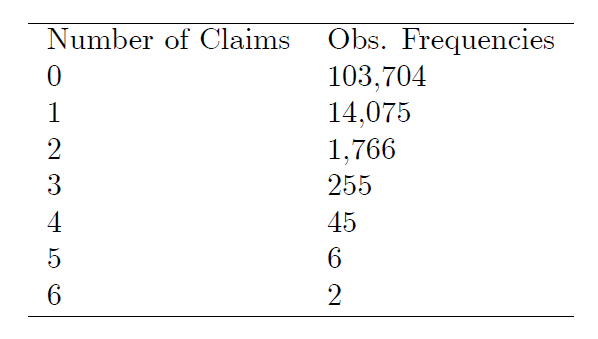
\includegraphics[width=0.4\textwidth]{2025-09-08 155257}
    % \caption{This is a sample figure caption}
    % \label{fig:example}
    \end{figure}
    \par To see whether the Poisson distribution fits the data, 
    we shall fit the data first under Poisson distribution with the 
    unknown parameter $\lambda$ estimated by using Maximum Likelihood Estimation.



    }
    
\end{frame}
\section{A Data Set}
\begin{frame}{A Data Set Con.}

    {\footnotesize \footnotesize
    \par  Consider i.i.d. samples $A_i$, $i=1,2,...,n$, from a Poisson distribution with rate $\lambda$. We want to estimate $\lambda$. 
    The likelihood is given by:
    \[
    L(\lambda) = \prod_{i=1}^{n} e^{-\lambda} \frac{\lambda^{A_i}}{A_i!}.
    \]
    \par Therefore, the log-likelihood is:
    \[
    \log L(\lambda) = \sum_{i=1}^{n} \{ - \lambda + A_i \log (\lambda) - \log (A_i!) \} 
    = -n \lambda + \log (\lambda) \sum_{i=1}^{n} A_i - \sum_{i=1}^{n} \log (A_i!)
    \]
    \par Taking derivatives with respect to $\lambda$ and then setting them to zero yield:
    \[
    -n + \frac{\sum_{i=1}^n A_i}{\lambda} = 0
    \]
    \par Therefore, the estimators for $\lambda$ is $\hat{\lambda} = \frac{1}{n} \sum\limits_{i=1}^n A_i.$


    }
    
\end{frame}
\begin{frame}{A Data Set Con.}

    {\footnotesize \footnotesize
    \par  In our example of the accident claims in 1961 for a class of automobile insurance by firms in Switzerland, we have:
    \[
    \hat{\lambda} = \frac{1}{n} \sum_{i=1}^n A_i
    \]
    \[
    = \frac{1}{n} \left\{ 0 \times 103,704 + 1 \times 14,075 + 2 \times 1,766 + 
    3 \times 255 + 4 \times 45 + 5 \times 6 + 6 \times 2 \right\}
    \]
    \[
    = 0.15514
    \]
    \par where the total sample size is:
    \[
    n = 103704 + 14075 + 1766 + 255 + 45 + 6 + 2 = 119853
    \]
    \par Therefore, the fitted model for zero claims is:
    \[
    n \times \left( e^{-\hat{\lambda}} \frac{\hat{\lambda}^0}{0!} \right) = 
    119853 \times e^{-\hat{\lambda}} = 119853 \times e^{-0.15514} = 102629.6
    \]

    

    }
    
\end{frame}

\begin{frame}{A Data Set Con.}


    {\footnotesize \footnotesize
    \par We can continue to get all the fitted values for one claim, two claims, 
    etc. The fitted model can be summarized in the following table.
    \begin{figure}
    \centering
    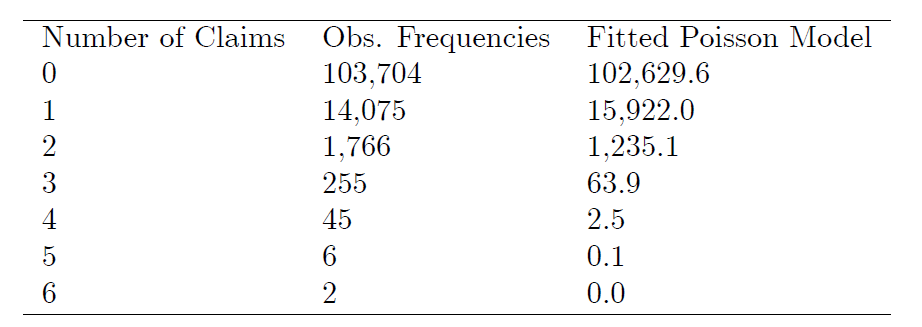
\includegraphics[width=0.6\textwidth]{2025-09-08 155325}
    % \caption{This is a sample figure caption}
    % \label{fig:example}
    \end{figure}
    \par Note that the Poisson process fts the tail part of the data rather poorly.
    Next, we shall discuss how to fit models to data better using an alternative
    model.
    }
    
\end{frame}

\section{Pólya counting process}
\begin{frame}{Pólya counting process}

    {\footnotesize \footnotesize
    \par To get a better fit of the data, we shall consider the Pólya counting process,
    which is a generalization of the Poisson process.
    \vspace{1em}

    \par The Pólya counting process $N(t)$ has a negative binomial distribution:
    \begin{align*}
        P(N(t) = i) = \binom{a + i - 1}{i}
         \left( \frac{b}{t + b} \right)^a \left( \frac{t}{t + b} \right)^i, 
         \quad t \geq 0, \quad i \geq 0, \quad a > 0, \quad b > 0
    \end{align*}
    \par Note that \( a > 0 \) is not necessarily an integer, where the binomial coefficients for non-integers are defined as:

    \[
    \binom{x}{y} = \frac{\Gamma(x + 1)}{\Gamma(y + 1)\Gamma(x - y + 1)}
    \]

    \par via the gamma function.

        }
\end{frame}


\begin{frame}{Pólya counting process Con.}

    {\footnotesize \footnotesize
    \par The Pólya counting process is a generalization of Poisson processes, because it is a mixed Poisson process with the rate \( \lambda \) is a random variable \( \Lambda \) with a gamma density

    \[
    \frac{b^a}{\Gamma(a)} e^{-bx}x^{a-1}
    \]

    \par where \( \Gamma(a) \) is a gamma function.
    
    \vspace{1em}
    \par The properties of the Pólya counting process:
    \vspace{1em}
    \par (1) Stationary but dependent increments. The Pólya counting process
    has a property that the arrival of one event tends to trigger more arrival events,
    leading to the positive correlation of increments. Indeed, $\text{Cov}(N(t),\ N(t+h)-N(t)) = ht\text{Var}(\Lambda) = ht\frac{a}{b^{2}}.$
    \par [Proof]
    \begin{align*}
        E[N(t)(N(t+h)-N(t))] &= E[E[N(t)(N(t+h)-N(t))|\Lambda]]\\ 
        &= E[t\Lambda\cdot h\Lambda]\\&= th\cdot E[\Lambda^{2}]
    \end{align*}

    }
    
\end{frame}

\begin{frame}{Pólya counting process Con.}

    {\footnotesize \footnotesize
    \par Therefore:

    \[
    \begin{aligned}
    &\text{Cov}(N(t),\ N(t+h)-N(t)) \\
    &= E[N(t)(N(t+h)-N(t))]-E[N(t)]E[(N(t+h)-N(t))] \\
    &= thE[\Lambda^{2}]-thE[\Lambda]E[\Lambda] = th\text{Var}(\Lambda)
    \end{aligned}
    \]
    \par Due to dependent increments, it is more challenging to analyze the Pólya counting process.
    \vspace{1em}
    \par (2) The Pólya counting process is a pure birth process with a birth rate being:

    \[
    q_{i,i+1}(t) = \frac{a+i}{b+t},
    \]

    \par where \(a\) and \(b\) are two parameters in the negative binomial distribution. 
    This fact may be helpful when one tries to simulate the Pólya counting process.
    

    }
    
\end{frame}

\begin{frame}{Estimation}

    {\footnotesize \footnotesize
    \par  It is challenging to get the maximum likelihood estimators for \(a\) and \(b\), involving infinite series 
    and two implicit equations. However, it is easier to get estimators via the method of moments. Oberve that:

    \[
    E\left[N(t)\right]=\frac{at}{b},\quad \text{Var}\left[N(t)\right]=a\frac{t}{b}\left(1+ \frac{t}{b}\right)
    \]

    \par Setting up two equations

    \[
    \frac{at}{b}=\bar{X},\quad a\frac{t}{b}\left(1+\frac{t}{b}\right)=S^{2}
    \]

    \par yields

    \[
    \hat{a}=\frac{(\bar{X})^{2}}{S^{2}-\bar{X}},\quad \hat{b}=\frac{t}{(S^{2}/\bar{X})-1}
    \]

    }
    
\end{frame}

\begin{frame}{Estimation Con.}

    {\footnotesize \footnotesize
    \par In our example, $\sum X_{i}=18594,\;\sum X_{i}^{2}=24376,\; n=119853,\;t=1.$ So:
    \[
    \bar{X}=0.1551400466,\quad S^{2}=0.1793155390.
    \]
    % \vspace{-0.5em}
    \par Thus:
    % \vspace{-0.5em}
    \[
    \hat{a}=0.9955716169,\quad \hat{b}=6.417244540
    \]
    \par Using the estimator \(\hat{a}\) and \(\hat{b}\) we get the following table for the negative binomial model.
    \begin{figure}
    \centering
    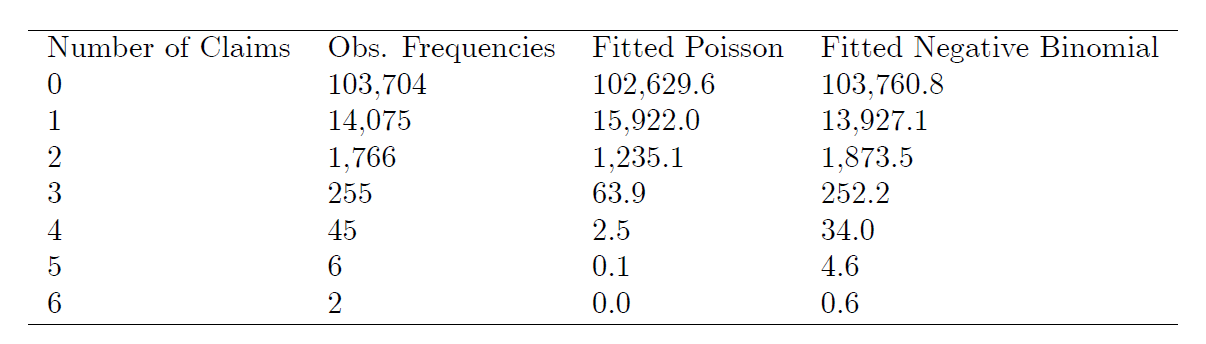
\includegraphics[width=0.6\textwidth]{2025-09-08_1}
    % \caption{This is a sample figure caption}
    % \label{fig:example}
    \end{figure}
    \par The negative binomial model fits the data better than the Poisson model,
    especially in the tail part.
    }
    
\end{frame}

\section{Introduction to Jump Diffusion Processes}
\begin{frame}{Introduction to Jump Diffusion Processes}

    {\footnotesize \footnotesize
    \par A finite-activity jump process $J(t)$ is a process such that:
    \begin{itemize}
        \item (i) \( J(t) \) is right-continuous. 
        At a jump time \( t \), \( J(t-) \) is the value just before the jump, \( J(t) \) is just after.
        \item (ii) There is no jump at time t, i.e. \( J(t-) = J(t) \).
        \item (iii) Finite number of jumps in any finite interval. In other words, there is only a finite number of points such that \( J(t-) \neq J(t) \).
    \end{itemize}
    \vspace{1em}
    \par These assumptions make stochastic 
    calculus with jumps easier than with infinite-activity processes. Consider a stochastic process: 

        \[
        X(t) = X(0) + \int_{0}^{t} \theta(s) dW(s) + \int_{0}^{t} \mu(s) ds + J(t).
        \]

    \par We can also write this as $X(t) = X^{c}(t) + J(t)$, where:
    

    \[
    X^{c}(t) = X(0) + \int_{0}^{t} \theta(s) dW(s) + \int_{0}^{t} \mu(s) ds
    \]

    \par is the part with a continuous sample path.

    }
\end{frame}

\section{The Definition of Stochastic Integral}
\begin{frame}{The Definition of Stochastic Integral}

    {\footnotesize \footnotesize
    \par We can define the stochastic integral \(\int_0^t \pi(s) dX(s)\). If \(\pi(t) \in \mathcal{F}_t\) and \(\pi(t)\) is left-continuous then the definition is given by
    \[
    \int_0^t \pi(s) dX(s) = \int_0^t \pi(s) \theta(s) dW(s) + \int_0^t \pi(s) \mu(s) ds + \sum_{0 < s \leq t} \pi(s) \Delta J(s),
    \]
    \par or we can denote in differential form
    \[
    \pi(t) dX(t) = \pi(t) \theta(t) dW(t) + \pi(t) \mu(t) dt + \pi(t) \Delta J(t).
    \]

    \par Note that the sum is only active for the finite number of terms.
    \vspace{1em}
    \par If \( X(t) \) is a martingale, then under suitable integrability:
    \[
    \mathbb{E} \left[ \int_{0}^{t} \pi^2(s) \theta^2(s) \, ds \right] < \infty
    \]
    \par The stochastic integral \(\int_{0}^{t} \pi(s) \, dX(s)\) is also a martingale. \( \pi(t) \) 
    must be predictable (left-continuous). Otherwise, the martingale property may fail.

    }
    
\end{frame}

\section{Itô Formula}
 \begin{frame}{Itô Formula}

    {\footnotesize \footnotesize
    \par Recall Itô formula without jumps, for a continuous semimartingale \( X^c(t) \):
    \[
    f(X^c(t)) = f(X^c(0)) + \int_0^t f'(X^c(s)) \, dX^c(s) + \frac{1}{2} \int_0^t f''(X^c(s)) \, d[X^c(s), X^c(s)]
    \]
    \par The Itô formula for a jump process \( X(t) \):
    \begin{align*}
        f(X(t)) = f(X(0)) + &\int_{0}^{t} f'(X(s))dX^{c}(s) 
        + \frac{1}{2}\int_{0}^{t} f''(X(s))d[X^{c}(s), X^{c}(s)]\\
        & + \sum_{0<s\leq t}[f(X(s)) - f(X(s-))]
    \end{align*}
    \par Denote $\Delta f(X(s)) = f(X(s)) - f(X(s-))$.
    \vspace{1em}
    \par The Itô formula in differential form: 

    \[
    df(X(t)) = f'(X(t))dX^{c}(t) + \frac{1}{2}f''(X(t))d[X^{c}(t), X^{c}(t)] + \Delta(f(X(t)))
    \]
    }
    
\end{frame}

 \begin{frame}{Itô Formula Con.}

    {\footnotesize \footnotesize
    \par Consider a jump-diffusion process for the return processes:

    \[
    X(t) = X(0) + (\mu - \frac{1}{2} \sigma^2)t + \sigma W(t) + \sum_{i=1}^{N(t)} \ln(V_i).
    \]

    \par Then the stock price \( S(t) = e^{X(t)} \) is given by:
    \begin{align*}
        S(t) = e^{X(t)} = S(0) \exp \left\{ (\mu - \frac{1}{2} \sigma^2)t 
        + \sigma W(t) \right\} \prod_{i=1}^{N(t)} V_i
    \end{align*}
    \par Now apply Itô formula to \( e^{X(t)} \), we have:

    \[
    \begin{aligned}
    dS(t) &= e^{X(t)} d \left\{ (\mu - \frac{1}{2} \sigma^2)t + \sigma W(t) \right\} + \frac{1}{2} \sigma^2 e^{X(t)} dt + \Delta S(t) \\
    &= (\mu - \frac{1}{2} \sigma^2) S(t) dt + S(t) \sigma dW(t) + \frac{1}{2} \sigma^2 S(t) dt + \Delta S(t) \\
    &= \mu S(t) dt + S(t) \sigma dW(t) + \Delta S(t)
    \end{aligned}
    \]
    }
    
\end{frame}

 \begin{frame}{Itô Formula Con.}

    {\footnotesize \footnotesize
    \par Example 1: Consider a jump-diffusion process for the return processes:

    \[
    X(t) = X(0) + (\mu - \frac{1}{2} \sigma^2)t + \sigma W(t) + \sum_{i=1}^{N(t)} \ln(V_i).
    \]

    \par Then the stock price \( S(t) = e^{X(t)} \) is given by:
    \begin{align*}
        S(t) = e^{X(t)} = S(0) \exp \left\{ (\mu - \frac{1}{2} \sigma^2)t 
        + \sigma W(t) \right\} \prod_{i=1}^{N(t)} V_i
    \end{align*}
    \par Now apply Itô formula to \( e^{X(t)} \), we have:

    \[
    \begin{aligned}
    dS(t) &= e^{X(t)} d \left\{ (\mu - \frac{1}{2} \sigma^2)t + \sigma W(t) \right\} + \frac{1}{2} \sigma^2 e^{X(t)} dt + \Delta S(t) \\
    &= (\mu - \frac{1}{2} \sigma^2) S(t) dt + S(t) \sigma dW(t) + \frac{1}{2} \sigma^2 S(t) dt + \Delta S(t) \\
    &= \mu S(t) dt + S(t) \sigma dW(t) + \Delta S(t)
    \end{aligned}
    \]
    }
    
\end{frame}

 \begin{frame}{Itô Formula Con.}

    {\footnotesize \footnotesize
    \par Now we need to compute \(\Delta S(t)\). Suppose the \(i\)th jump occur at time \(t\), 
        the change in \(S\) is from \(S(t-)\) to \(S(t-)V_i\).
     Therefore, the change is \(S(t-)V_i - S(t-) = S(t-)(V_i - 1)\). 
     \par In this case, at the \(i\)th jump time \(t\) is \(V_i - 1\), which can also be written more generally as

    \[
    V_i - 1 = d \left( \sum_{i=1}^{N(t)} (V_i - 1) \right)
    \]
    \vspace{1em}
    \par Which interpret as increment of the cumulative process at time t is equal to the jump size at t. 
    Therefore, without referring to the specific jump time, we have: 
    \begin{align*}
        \Delta S(t) = S(t-)d \left( \sum_{i=1}^{N(t)} (V_i - 1) \right)
    \end{align*}
    }
    
\end{frame}

\begin{frame}{Itô Formula Con.}

    {\footnotesize \footnotesize
    \par Since in continuous parts of the trajectory (no jump), $S(t) = S(t-)$. In summary, we have: 

    \[
    \begin{aligned}
    dS(t) &= \mu S(t)dt + S(t)\sigma dW(t) + S(t-)d \left( \sum_{i=1}^{N(t)} (V_i - 1) \right) \\
    &= \mu S(t-)dt + S(t-)\sigma dW(t) + S(t-)d \left( \sum_{i=1}^{N(t)} (V_i - 1) \right)
    \end{aligned}
    \]

    \par or

    \[
    \frac{dS(t)}{S(t-)} = \mu dt + \sigma dW(t) + d \left( \sum_{i=1}^{N(t)} (V_i - 1) \right)
    \]
    }
    
\end{frame}


\begin{frame}{Itô Formula Con.}

    {\footnotesize \footnotesize
    \par Example 2: Suppose  
    \[
    \frac{dZ(t)}{Z(t-)} = \mu_0 dt + \sigma dW(t) + d \left[ \sum_{i=1}^{N(t)} (V_i - 1) \right], \quad Z(0) = 1
    \]
    \par where  
    \[
    \mu_0 = -\lambda E[V - 1]
    \]
    \par Then we shall show that \(Z(t)\) is a martingale. We know from Example 1 that:
    \[
    Z(t) = \exp \left\{ -\frac{1}{2} \sigma^2 t + \sigma W(t) \right\} e^{\mu_0 t} \prod_{i=1}^{N(t)} V_i
    \]
    \par But  
    \[
    E \left[ \prod_{i=1}^{N(t)} V_i \middle| \mathcal{F}_s \right] 
    = \prod_{i=1}^{N(s)} V_i \cdot E \left[ \prod_{i=N(s)+1}^{N(t)} V_i \right]
    \]
    }
    
\end{frame}

\begin{frame}{Itô Formula Con.}

    {\footnotesize \footnotesize
    \par However

    \[
    \begin{aligned}
    E \left[ \prod_{i=N(s)+1}^{N(t)} V_i \right] 
    &=\sum_{n=0}^{\infty} \mathbb{E} \left[ \prod_{i=1}^{n} V_i \middle| N(t)-N(s) = n \right] \cdot \text{P}(N(t)-N(s) = n)\\
    &= \sum_{n=0}^{\infty} e^{-\lambda (t-s)} \frac{(\lambda (t-s))^n}{n!} E \left[ \prod_{i=0}^{n} V_i \right] \\
    &= \sum_{n=0}^{\infty} e^{-\lambda (t-s)} \frac{(\lambda (t-s))^n}{n!} (E [V])^n \\
    &= e^{-\lambda (t-s)} \sum_{n=0}^{\infty} \frac{(\lambda E [V] (t-s))^n}{n!} \\
    &= e^{-\lambda (t-s)} e^{\lambda E [V] (t-s)} \\
    &= e^{-\mu_0 (t-s)}
    \end{aligned}
    \]
    }
    
\end{frame}


\begin{frame}{Itô Formula Con.}

    {\footnotesize \footnotesize
    \par which show that for any $s<t$:
    \[
    \begin{aligned}
    E [Z(t) | \mathcal{F}_s] &= E \left[ \exp \left\{ -\frac{1}{2} \sigma^2 t + \sigma W(t) \right\} e^{\mu_0 t} \prod_{i=1}^{N(t)} V_i \middle| \mathcal{F}_s \right] \\
    &= Z(s) E \left[ \exp \left\{ -\frac{1}{2} \sigma^2 (t-s) + \sigma (W(t) - W(s)) \right\} e^{\mu_0 (t-s)} \prod_{i=N(s)+1}^{N(t)} V_i \middle| \mathcal{F}_s \right] \\
    = &Z(s) E \left[ \exp \left\{ -\frac{1}{2} \sigma^2 (t-s) + \sigma (W(t) - W(s)) \right\}\right]\cdot
    E \left[ e^{\mu_0 (t-s)} \prod_{i=N(s)+1}^{N(t)} V_i \middle| \mathcal{F}_s \right] \\
    &= Z(s)
    \end{aligned}
    \]

    }
    
\end{frame}

\section{Girsanov Theorem}
\begin{frame}{Girsanov Theorem}

    {\footnotesize \footnotesize
    \par If we use \( Z(t) \) in Example 2, i.e.

\[
\frac{dZ(t)}{Z(t-)} = \mu_0 dt + \sigma dW(t) + d \left[ \sum_{i=1}^{N(t)} (V_i - 1) \right], \quad Z(0) = 1
\]

to define a new probability measure \( P^* \) via $\frac{dP^*}{dP} = Z(t).$ 
Then Girsanov theorem says that under \( P^* \):
\begin{itemize}
    \item $W^*(t) = W(t) - \sigma t$ is a standard Brownian motion.
    \item The new jump density of \( V \) is given by $f_V^*(x) = \frac{1}{E[V]} x f_V(x)$.
    \item The new jump rate is given by $\lambda^* = \lambda E[V]$.
\end{itemize}
\vspace{1em}
\par Instead of giving rigorous proof of the theorem, we present a heuristic derivation. 
First of all, \( W^*(t) \) is a new Brownian motion due to the standard Girsanov theorem for Brownian motion. Thus, we shall focus on the jump part.
    }
    
\end{frame}

\begin{frame}{Girsanov Theorem Con.}

    {\footnotesize \footnotesize
    \par Consider the jump arrival times $\tau_1, ..., \tau_n, ...,$ and the related jump sizes $V_1, V_2, ...,$. 
    Conditioning on the event that $\{\tau_n \in [t, t + dt]\}$, we have the jump intensity under the old measure $P$ is given by:
    \begin{align*}
        \lambda(dt, dx) := P(\tau_n \in [t, t + dt],  V_n \in [x, x + dx] | \mathcal{F}_{t-}) = \lambda dt \cdot f_V(x) dx
    \end{align*}
    \par This means that a jump happens in \([t, t + dt]\) with probability about \(\lambda dt\) and 
    conditional on a jump, the size distribution is \(f_V(x)\). By the Bayes formula for the measure transform, we have the new intensity:

    \[
    \begin{aligned}
    \lambda^*(dt, dx) &= P^*(\tau_n \in [t, t + dt],  V_n \in [x, x + dx] | \mathcal{F}_{t-}) \\
    &= E^*[I(\tau_n \in [t, t + dt]) I(V_n \in [x, x + dx]) | \mathcal{F}_{t-}] \\
    &= E \left[ \frac{Z(t)}{Z(t-)} \cdot I(\tau_n \in [t, t + dt]) I(V_n \in [x, x + dx]) | \mathcal{F}_{t-} \right]
    \end{aligned}
    \]
    \par Conditioning on the event that $\{\tau_n \in [t, t + dt]\}$, \( Z(t) \) is updated by a multiplicative factor \( V_n \):

    \[
    \frac{Z(t)}{Z(t-)} = V_n
    \]
    }
    
\end{frame}

\begin{frame}{Girsanov Theorem Con.}

    {\footnotesize \footnotesize
    \par which yields:
    \[
    \begin{aligned}
    \lambda^*(dt, dx) &= E \left[ E \left\{ \frac{Z(t)}{Z(t-)} \cdot I(\tau_n \in [t, t + dt]) I(V_n \in [x, x + dx]) | \tau_n \in [t, t + dt] \right\} \middle| \mathcal{F}_{t-} \right] \\
    &= E \left[ E \left\{ V_n I(\tau_n \in [t, t + dt]) I(V_n \in [x, x + dx]) \middle| \tau_n \in [t, t + dt] \right\} \middle| \mathcal{F}_{t-} \right] \\
    &= E \left[ I(\tau_n \in [t, t + dt]) E \{ V_n I(V_n \in [x, x + dx]) | \tau_n \in [t, t + dt] \} | \mathcal{F}_{t-} \right] \\
    &= E \left[ I(\tau_n \in [t, t + dt] | \mathcal{F}_{t-}) \right] \cdot E \{ V_n I(V_n \in [x, x + dx]) | \mathcal{F}_{t-} \} \\
    &= \lambda dt \cdot E \left[ V_n I(V_n \in [x, x + dx]) | \mathcal{F}_{t-} \right],
    \end{aligned}
    \]
    \par via independence. Thus:
    \[
    \begin{aligned}
    \lambda^*(dt, dx) &= \lambda dt \cdot x f_V(x) dx = (E [V] \lambda) dt \cdot \frac{x f_V(x)}{E [V]} dx
    \end{aligned}
    \]

which is the jump intensity of a new jump diffusion process with jump rate $\lambda^* = E [V] \lambda$, and jump size density:

\[
\frac{x f_V(x)}{E [V]}, \;\;\; \text{with} \int_{0}^{\infty} \frac{x f_V(x)}{E[V]}  dx =  1
\]

where the normalizing constant $E [V]$ is needed to get a proper density function.

    }
    
\end{frame}

% \begin{frame}

%     {\footnotesize \footnotesize

%     }
    
% \end{frame}
% % {\mathbb{P}^*}
% \tilde{\mathbb{P}}
% {\footnotesize \footnotesize
% }
% \tiny
% \scriptsize
% \footnotesize
% \small
% \normalsize (default)
% \large
% \Large
% \LARGE
% \huge
% \Huge
\end{document}